\documentclass[wmii, inf, inz]{uwmthesis}
\usepackage[polish]{babel} \usepackage[utf8]{inputenc}
\usepackage[T1]{fontenc}
\usepackage[utf8]{inputenc}
\usepackage[MeX]{polski}
\usepackage{url}
\usepackage{tikz}
\usepackage{pgfplots}
\usepackage{pgfplotstable}
\usepackage{lmodern}
\usepackage{cleveref}
\usepackage{geometry}
\newgeometry{tmargin=2.5cm, bmargin=2.5cm, lmargin=3.5cm, rmargin=2cm}
\pgfplotsset{compat=1.16}
\widowpenalty10000  
\clubpenalty10000 
\linespread{1.1}
\date{2019}
\title{Symulacja ruchu drogowego na skrzyżowaniu z~sygnalizacją świetlną sterowaną algorytmem ewolucyjnym}
\author{Krzysztof Pietraszko}
\etitle{Traffic simulation on junction with traffic lights controlled by an evolutionary algorithm}
\wykonanaw{Katedrze Metod Matematycznych Informatyki}
\ewykonanaw{the Department of Mathematical Methods in Computer Science}

\podkierunkiem{Dr Inż. Bartosza Nowaka}
\epodkierunkiem{Dr Inż. Bartosz Nowak}

\begin{document}
	\pgfplotstableread[col sep = comma]{evolutionLog.csv}\loadedtable
	\maketitle
	\chapter*{Streszczenie}
	\chapter*{Abstract}
The goal of the thesis was to implement an evolutionary algorithm that optimises traffic lights on a junction. \\
Evolutionary algorithms are a category of artificial intelligence techniques. They are widely used to solve optimisation problems. Their main mechanisms are inspired by the evolution of species. \\
Traffic lights improvement was presented as an optimisation problem with a goal function dependant on a simulation of the traffic. Unity engine and C\texttt{\#} language were used to implement the application. It performs the optimisation process with settings provided by the user. This thesis describes the algorithm and the functionality of the application itself. The results of optimisation were presented in the form of charts. Possible directions for further extension of the application were also proposed.
	\tableofcontents
	\chapter*{Wstęp}
%Wstęp od stworzenia swiata: komputery są pomocne również w zadaniach inżynieryjnych takich jak problemy optymalizacyjne np problem ustawienia optymalnych czasów (jak to ująć?)
\paragraph{}Komputery są obecnie niezwykle popularnymi urządzeniami znajdującymi zastosowanie w wielu dziedzinach życia. Są pomocne także w zadaniach inżynieryjnych takich jak problemy optymalizacyjne.
\section*{Problemy optymalizacyjne}
Problemy w wielu obszarach matematyki, inżynierii, ekonomii, medycyny i statystyki mogą być przedstawione w kategoriach optymalizacji.\\
Określenie problemu optymalizacyjnego rozpoczyna się od ustalenia zbioru zmiennych niezależnych lub parametrów. Często formułuje się również ograniczenia, które wyznaczają dozwolone wartości zmiennych. Inną istotną składową problemu optymalizacyjnego jest funkcja celu, której wartość zależy od zmiennych. Rozwiązaniem takiego problemu jest zbiór dozwolonych wartości zmiennych, dla których funkcja przyjmuje optymalną wartość (minimalną lub maksymalną, zależnie od badanego zagadnienia)\cite{9780122839528}.
\paragraph{} Do rozwiązywania problemów optymalizacyjnych często stosowane są metody sztucznej inteligencji. Dostarczają lepszych, szybszych i bardziej precyzyjnych rozwiązań niż konwencjonalne techniki, szczególnie w złożonych problemach inżynieryjnych. Spośród ich charakterystycznych cech warto wymienić następujące:
\begin{itemize}
	\item Metody te ,,pamiętają'' swoje poprzednie odkrycia,
	\item Dostosowują swoją wydajność (np. decydują o eksploracji lub eksploatacji), co przekłada się na unikanie utknięcia w minimum lokalnym,
	\item Mogą planować swoje działania długofalowo~\cite{Badar2013StudyOA}.
\end{itemize}
\section*{Algorytmy ewolucyjne} Przykładowym typem metod sztucznej inteligencji są algorytmy ewolucyjne. Poszukują one optymalnego rozwiązania problemu w sposób, który czerpie inspirację z mechanizmu ewolucji gatunków. Jednym z głównych czynników wyróżniających ten zbiór technik jest to, że jednocześnie zmieniana jest pewna populacja rozwiązań, a jej przekształcenia przypominają procesy zachodzące w przyrodzie. Zrozumienie algorytmów ewolucyjnych wymaga przyswojenia pewnych kluczowych pojęć, takich jak dostosowanie (ang. \textit{fitness}) stanowiące ocenę danego rozwiązania, oraz krzyżowanie i mutacja będące mechanizmami przekształcania populacji. \\Krzyżowanie tworzy nowe rozwiązanie łącząc cechy dwóch innych, podczas gdy mutacja w losowy sposób modyfikuje istniejące rozwiązanie. 
Przebieg algorytmu genetycznego rozpoczyna się od utworzenia początkowej populacji rozwiązań, które zazwyczaj są generowane losowo. W związku z tym zakłada się, że jest to różnorodny zbiór zawierający dobre i złe cechy.
Algorytm następnie generuje szereg kolejnych populacji (pokoleń), z pomocą wyżej wspomnianych mechanizmów przekształcających~\cite{Cohoon:2003:EAP:903758.903786}. Kluczowe jest tu zachowanie równowagi między wykorzystywaniem znanych pozytywnych cech (a więc krzyżowaniem) a odkrywaniem nowych możliwości w przestrzeni dopuszczalnych rozwiązań (a więc mutacją). Istnieją modele mające na celu zmniejszenie tego problemu. Przykładowo działanie algorytmu można podzielić na fazy: pozyskiwania, akumulacji i wykorzystywania wiedzy~\cite{10.1371/journal.pone.0095693}. Innym rozwiązaniem jest przyjęcie zmiennego współczynnika mutacji danego pewną funkcją. Taką technikę przyjęto w tej pracy. 
\section*{Przykładowe zastosowania algorytmów ewolucyjnych} Do ciekawych zastosowań algorytmów ewolucyjnych należą m.in. antena statku kosmicznego~\cite{Lohn2006AutomatedAD}, czy też wentylator silnika~\cite{article}, których kształt został zaprojektowany przez taki algorytm. Obszary przejawiające duży potencjał to chociażby planowanie produkcji~\cite{Wall:1996:GAR:925320}, przewidywanie zmian temperatury na Ziemi\cite{Stanislawska:2012:MGT:2400749.2401077} i wiele innych~\cite{Steinbuch2010}.
\paragraph{}W tej pracy omówiono wykorzystanie algorytmu ewolucyjnego do usprawnienia płynności ruchu drogowego na skrzyżowaniu poprzez optymalizację sygnalizacji świetlnej. Stworzono aplikację przeprowadzającą proces uczenia z możliwością konfiguracji jego ustawień. Efektem końcowym pracy aplikacji jest wyświetlenie optymalnych parametrów sygnalizacji.
\section*{Usprawnienie sygnalizacji świetlnej jako problem optymalizacyjny}
Każda zmienna niezależna to czas, przez jaki wybrane sygnalizatory są zielone. Ewaluacja funkcji celu każdorazowo wymaga przeprowadzenia symulacji ruchu pojazdów, którą w tym celu zaimplementowano. Symulacja trwa dopóki określona liczba samochodów nie opuści skrzyżowania, a czas jej trwania decyduje o ocenie danego osobnika. \\
{\Huge TODO: OPIS ROZDZIAŁÓW}

	\chapter*{Użyte technologie}
Głównymi czynnikami decydującymi o doborze technologii były
\begin{itemize}
	\item Prostota interakcji z kartą graficzną,
	\item Dobre narzędzia do debugowania kodu,
	\item Jakość i kompletność dokumentacji,
	\item Wydajność,
	\item Możliwość prostej implementacji interfejsu graficznego,
	\item Wcześniejsze doświadczenie,
	\item Szybkość kompilacji -- istotna przy częstych zmianach w kodzie.
\end{itemize}
\section*{Unity}
Unity to wieloplatformowy silnik autorstwa firmy Unity Technologies, którego głównym zastosowaniem jest tworzenie gier dwuwymiarowych i trójwymiarowych oraz symulacji. W porównaniu do podobnych narzędzi wyróżnia się prostotą obsługi, dużym naciskiem na edytory wizualne i zintegrowanym środowiskiem, które nie wymaga skomplikowanej konfiguracji. Wspiera wiele API graficznych (DirectX, OpenGL, Metal i Vulkan)\cite{UnityManualGraphicsApiSupport} pod wspólnym interfejsem. Dzięki temu twórcy mogą w łatwy sposób tworzyć wersje swoich aplikacji na wiele platform bez uciążliwego dostosowywania swojego kodu. Podobne uproszczenia dostępne są również w zakresie obsługi urządzeń wejścia (jak mysz, klawiatura, kontrolery, ekrany dotykowe), a także dźwięku. Na wspomnienie zasługuje również wbudowany edytor WYSIWYG\footnote{WYSIWYG (What You See Is What You Get) - ,,otrzymujesz to co widzisz''} interfejsu graficznego aplikacji. Silnik można też rozszerzać o własne narzędzia, na przykład graficzny edytor krzywych. Programować swoją aplikację można jedynie w języku C\texttt{\#}~\cite{ProgramminginUnity}. Interfejs edytora Unity przedstawiono na rysunku~\ref{fig:unity}.
\section*{Język C\texttt{\#}}
C\texttt{\#} to silnie i statycznie typowany obiektowy język programowania zaprojektowany przez firmę Microsoft. Pozwala pisać kod z zachowaniem wszystkich założeń obiektowego paradygmatu programowania, czyli: abstrakcji, hermetyzacji, polimorfizmu i dziedziczenia. Mimo że C\texttt{\#} to język obiektowy, posiada wiele funkcji inspirowanych językami funkcyjnymi, które m.in. pozwalają bardzo łatwo dokonywać filtrowania, przekształcania czy sortowania kolekcji obiektów. Ułatwia to pisanie czytelnego, a przy tym zwięzłego, kodu. Pierwotnie kod C\texttt{\#} mógł być uruchamiany jedynie na systemie Windows. Zmieniło się to jednak w ostatnich latach dzięki środowiskom takim jak Mono oraz .NET Core i obecnie wspierane są inne platformy, takie jak Linux, macOS, iOS czy Android~\cite{Albahari2017}.
\begin{figure}[h!]
	\centering
	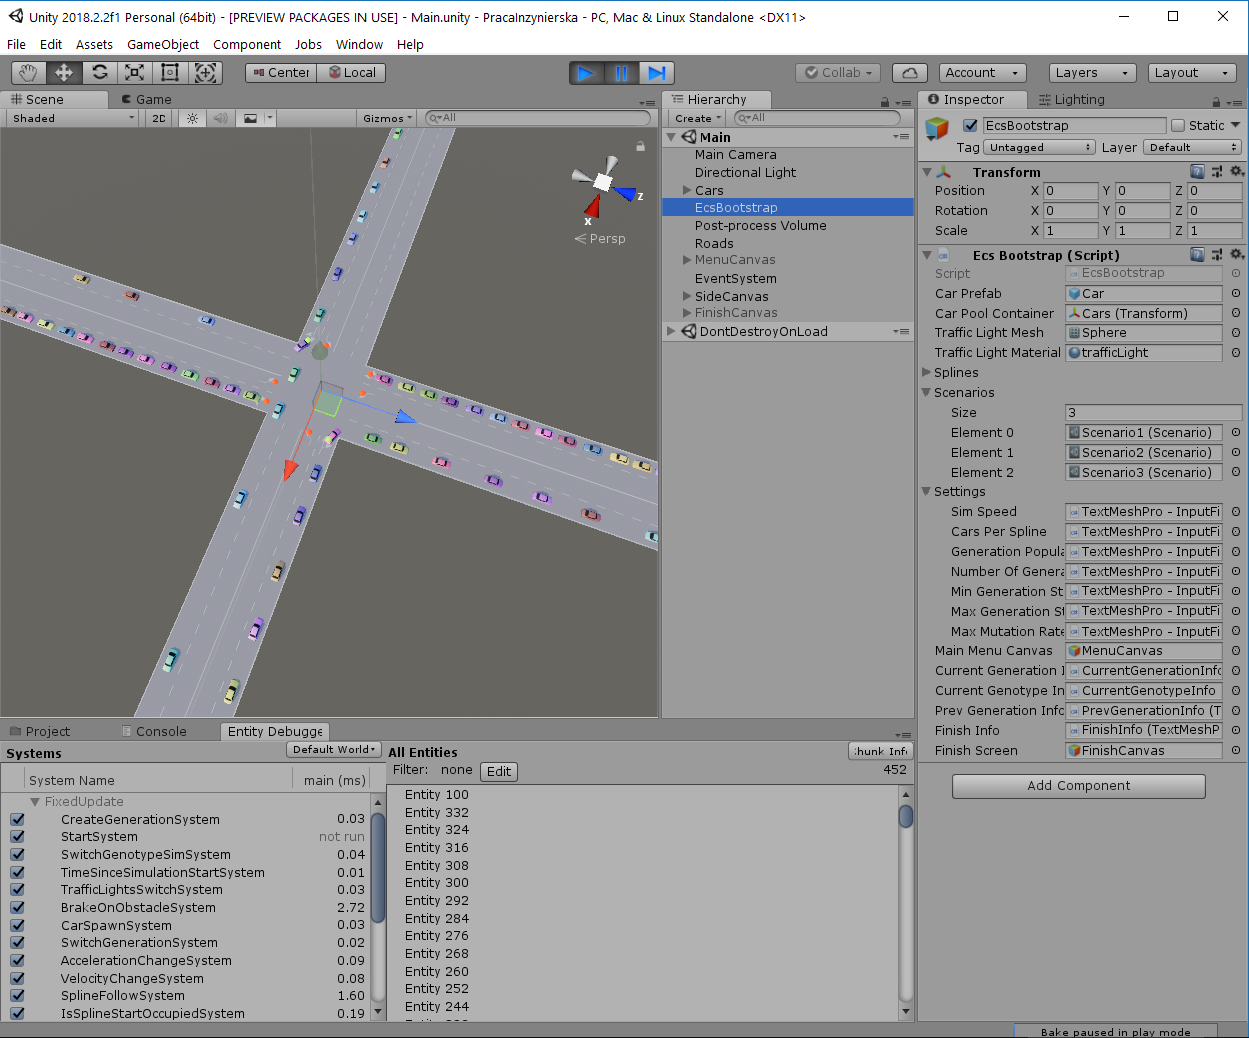
\includegraphics[width=1\linewidth]{unity}
	\caption[Interfejs edytora Unity]{Interfejs edytora Unity}
	\label{fig:unity}
\end{figure}
\section*{Inkscape}
Inkscape to darmowy program do tworzenia grafiki wektorowej. Tworząc w nim obrazy korzysta się z podstawowych kształtów takich jak elipsy, wielokąty, krzywe czy strzałki. Inkscape używa formatu Scalable Vector Graphics (SVG). Mimo że program opiera się na formacie wektorowym, plikiem wynikowym rysunku w tej pracy był obraz rastrowy, który można eksportować w dowolnej rozdzielczości. Decyzja ta wynika z ograniczeń w importowaniu grafik wektorowych w silniku Unity. Za użyciem Inkscape przemawiała przede wszystkim mnogość narzędzi i ustawień do tworzenia kształtów i wyrównywania ich położenia. Wygląd interfejsu programu przedstawiono na rysunku~\ref{fig:inkscape}. \\
W tej pracy został użyty do stworzenia grafiki skrzyżowania.
\begin{figure}
	\centering
	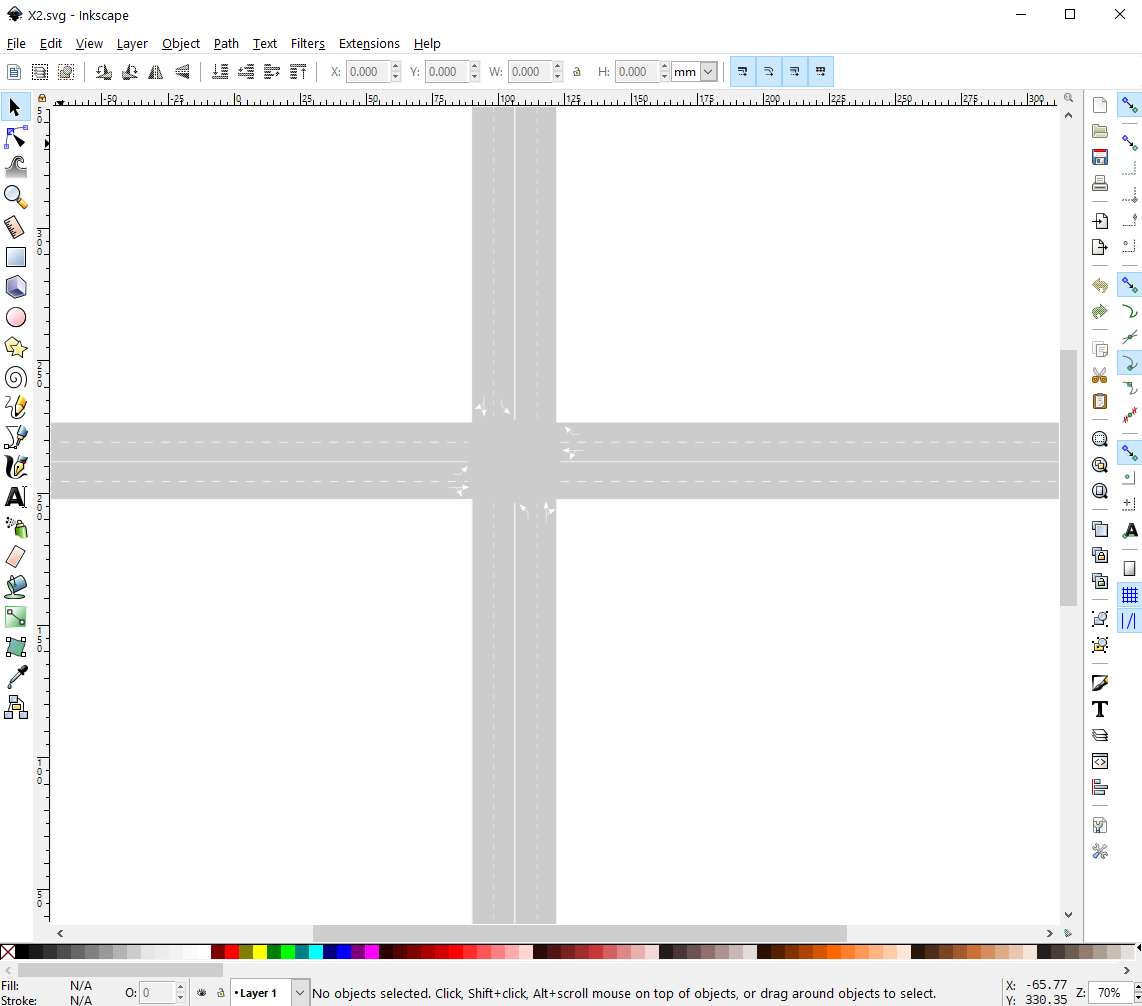
\includegraphics[width=1.0\linewidth]{inkscape}
	\caption[Interfejs programu Inkscape]{Interfejs programu Inkscape}
	\label{fig:inkscape}
\end{figure}
\section*{Blender}
Blender to darmowy program do tworzenia grafiki trójwymiarowej stworzony przez organizację Blender Foundation. Posiada narzędzia do modelowania, teksturowania, renderowania i animacji. Oprócz tego można z jego użyciem wykonywać proste symulacje fizyczne, a nawet zrealizować postprodukcję filmów. Niewątpliwie zaletą programu jest połączenie ogromnej liczby narzędzi w jeden pakiet. Dodatkowe atuty to dobra integracja z silnikiem Unity, wygoda użytkowania i wydajność. W tej pracy posłużył do wykonania trójwymiarowego modelu samochodu oraz ikony aplikacji. Interfejs Blendera przedstawia rysunek~\ref{fig:blender}.
\begin{figure}[h!]
	\centering
	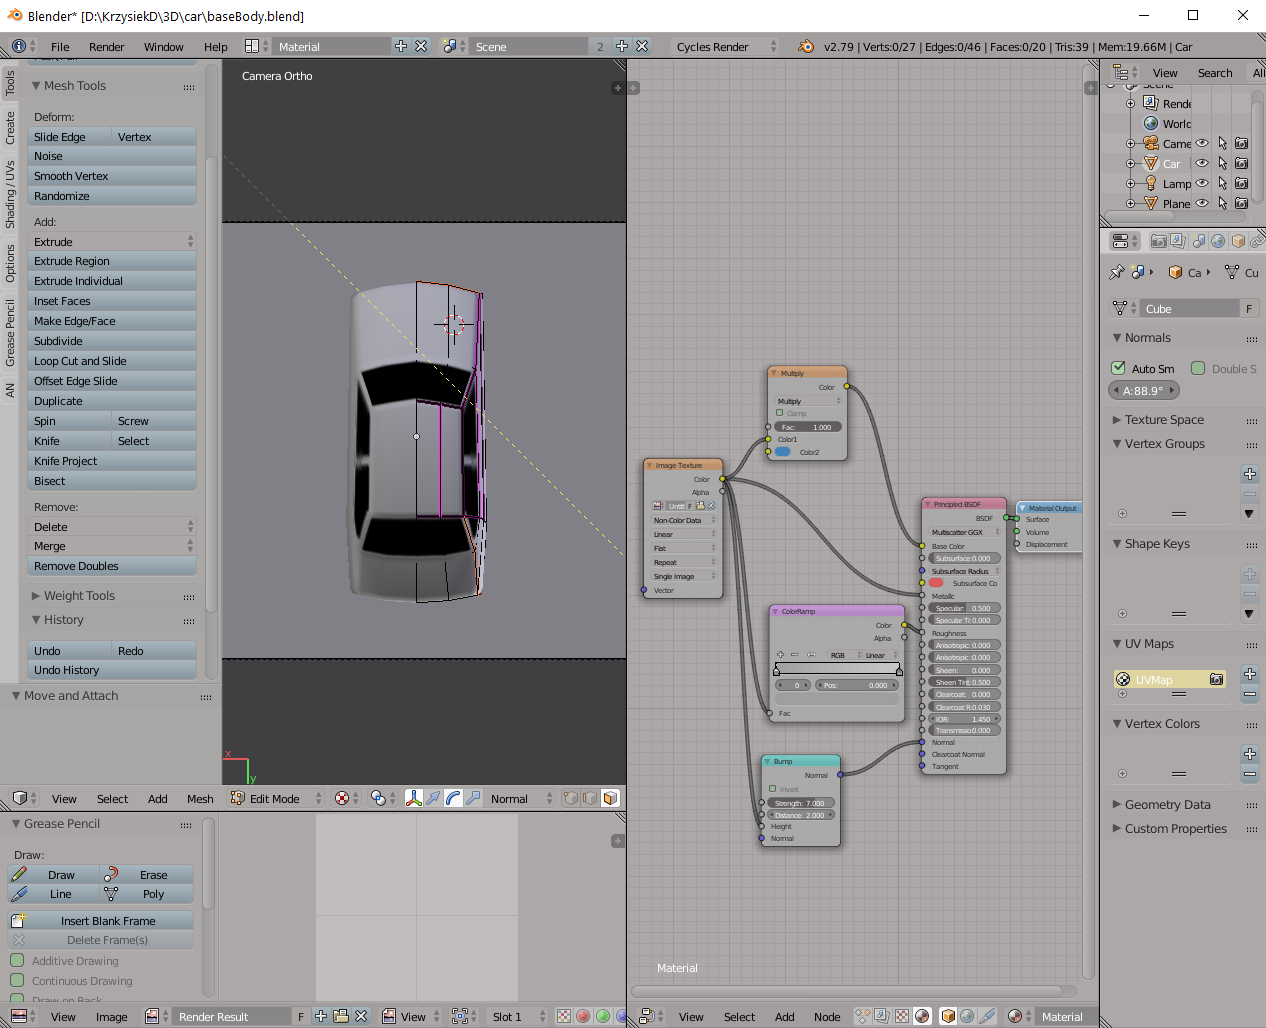
\includegraphics[width=1\linewidth]{blender}
	\caption[Interfejs programu Blender]{Interfejs programu Blender}
	\label{fig:blender}
\end{figure}


	\chapter*{Projekt aplikacji}
Aplikacja jest wysoce wyspecjalizowana -- przeprowadza wyłącznie proces symulacji i uczenia. Użytkownik może konfigurować ustawienia tego procesu.
\section*{Wymagania funkcjonalne}
\begin{itemize}
	\item Przeprowadzanie procesu uczenia optymalnych czasów świecenia sygnalizatorów na skrzyżowaniu za pośrednictwem algorytmu ewolucyjnego, wykorzystującego symulację ruchu pojazdów do oceny rozwiązań, 
	\item Konfiguracja ustawień symulacji, będącej bazą procesu uczenia,
	\item Konfiguracja ustawień algorytmu ewolucyjnego,
	\item Wyświetlanie na bieżąco informacji o przebiegu uczenia,
	\item Wyświetlenie wyników uczenia po jego zakończeniu.
\end{itemize}
\section*{Wymagania pozafunkcjonalne}
\begin{itemize}
	\item Stabilność -- aplikacja musi pracować bezawaryjnie przez wiele godzin,
	\item Wydajność -- aplikacja musi działać na tyle wydajnie, aby symulacja mogła być przeprowadzana kilkadziesiąt razy szybciej niż czas rzeczywisty.
\end{itemize}
\section*{Przypadki użycia}
W projekt występuje tylko jeden przypadek użycia: ,,Przeprowadź proces optymalizacji sygnalizacji świetlnej''. Przedstawia go diagram aktywności na rysunku~\ref{fig:diagramaktywnosci}. 
\section*{Przebieg przypadku użycia ,,Przeprowadź proces optymalizacji sygnalizacji świetlnej''}
Użytkownik najpierw może ustawić konfigurację symulacji oraz algorytmu ewolucyjnego. Następne wybiera scenariusz (czyli kolejność zapalania sygnalizatorów) co powoduje rozpoczęcie procesu uczenia. Aplikacja kolejno generuje, symuluje, a potem ocenia osobników pokolenia, jednocześnie wyświetlając na ekranie informacje o przebiegu uczenia. Pokolenia są kolejno generowane tak długo, aż zostanie osiągnięta ich liczba określona w konfiguracji. Następnie aplikacja wyświetla ekran końcowy prezentujący wyniki uczenia.
\begin{figure}[H]
	\centering
	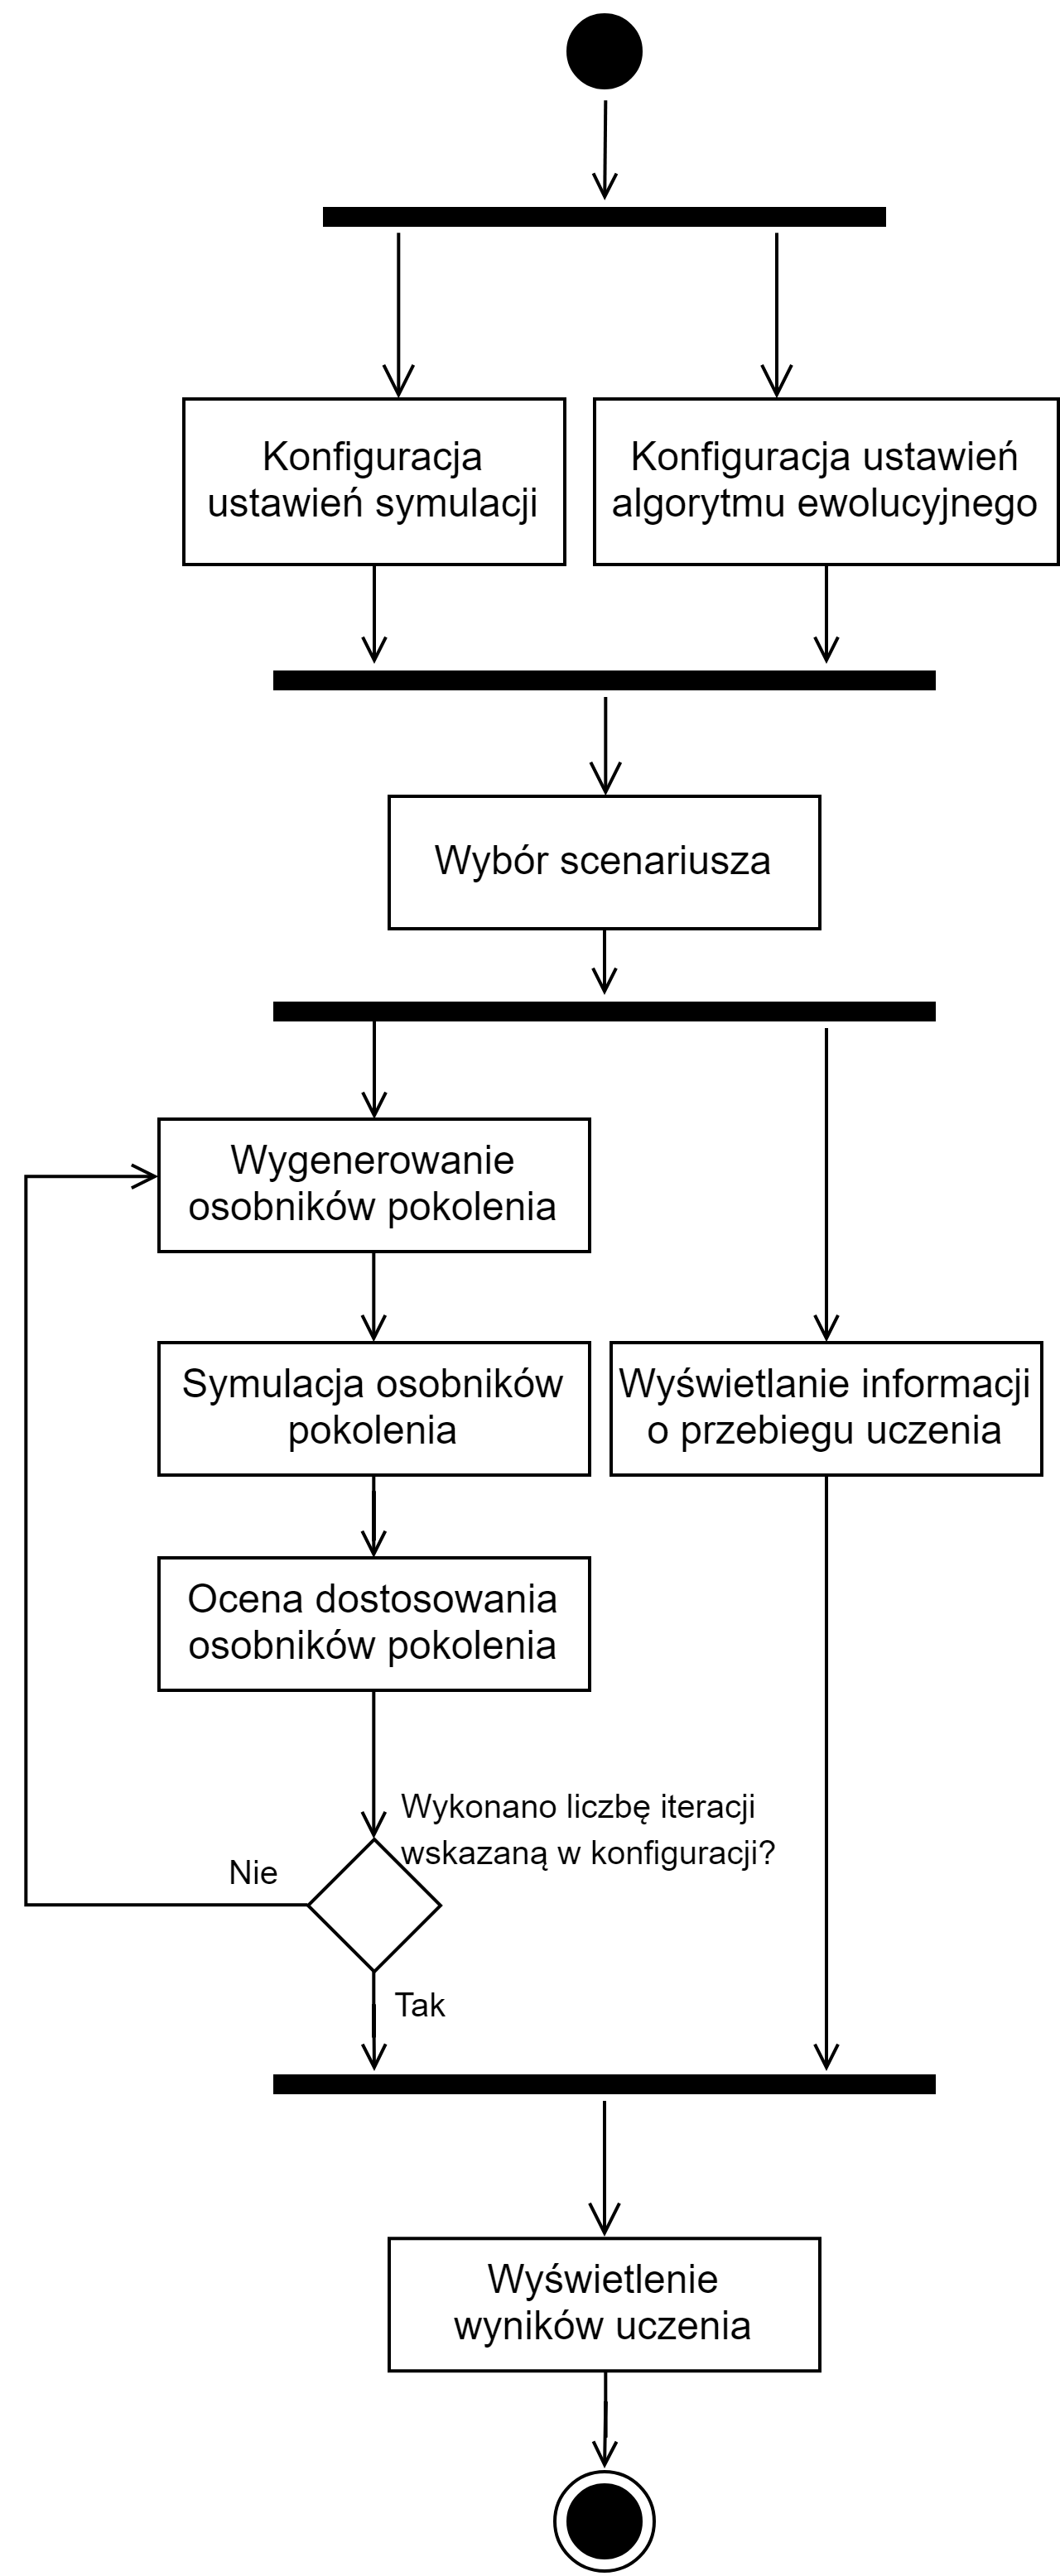
\includegraphics[height=0.8\textheight]{diagram_aktywnosci}
	\caption[Diagram aktywności przypadku użycia ,,Przeprowadź proces uczenia sygnalizacji'']{Diagram aktywności przypadku użycia ,,Przeprowadź proces uczenia sygnalizacji''}
	\label{fig:diagramaktywnosci}
\end{figure}

	\bibliographystyle{moj}
	\bibliography{bibliografia}
	\listoffigures
	
\end{document}